%----------------------------------------------------------------------------------
%----Präambel/Preamble-------------------------------------------------------------
%----------------------------------------------------------------------------------
\documentclass[	a4paper,
				11pt,
				DIV=11,
				bigheadings,
				idxtotoc,
				listof=totoc,	
				bibtotoc,		
				halfparskip,
				cleardoubleempty,
				oneside,
				openright]{scrartcl}
%----------------------------------------------------------------------------------

\usepackage[english]{babel}
\usepackage[T1]{fontenc}
\usepackage[utf8]{inputenc}
\usepackage{subfig}

\usepackage[OT1]{fontenc}
\renewcommand*\familydefault{\sfdefault}


\usepackage{graphicx}	

\usepackage[labelfont=bf]{caption}
					
\usepackage{float}
\usepackage{wrapfig}
%\usepackage{subfigure}

\usepackage{geometry}						% Für newgeometry in Titelseite
\geometry{a4paper,left=30mm,right=20mm}

\usepackage{blindtext}
\usepackage{layout}

\PassOptionsToPackage{hyphens}{url}		
\usepackage[pdfborder={0 0 0},
			colorlinks=true, 
			linkcolor=black,
			citecolor=red,
			]{hyperref}
			
\usepackage{natbib}%numbers 				

\usepackage{pdfpages}

\usepackage{color}
\usepackage{xcolor}

\usepackage{setspace}

\usepackage{longtable}
\usepackage{multirow}
\usepackage{colortbl}

%----------------------------------------------------------------------------------
%----Kopfzeile---------------------------------------------------------------------
%----------------------------------------------------------------------------------

\usepackage{scrlayer-scrpage} 							% Aufruf KOMA-Skript für Kopfzeilen

\pagestyle{scrheadings}							% Definition der Eigenen Headerformatierung
\clearscrheadfoot 								% alle Standard-Werte und Formatierungen raus
%\automark[chapter]{section}						% Kapitel und Section als Inhalt der Variablen leftmark und rightmark
\ohead{\pagemark}								% Seitenzahl auf äußerem Rand
\ihead{\ifthispageodd{\leftmark}{\rightmark}} 	% Innere Überschrift mit Kapitel bei linker Seite und Section bei rechter Seite -> geht nur in Verbindung mit
												% zweiseitigem Text wirklich sinnvoll
\setheadsepline{0.4pt} 							% Trennlinie Fußzeile und Textkörper
\setkomafont{pagehead}{\scshape}				% Schriftart in Kopfzeile, \scshape = Kapitelchen
%----Fußzeile----------------------------------------------------------------------
\setfootsepline{0.4pt} 							% Trennlinie Fußzeile und Textkörper
\setkomafont{pagefoot}{\scshape}				% Schriftart in Fußfzeile, \scshape = Kapitelchen
\ifoot{\footnotesize{Leong Eu Jinn}}
\ofoot{\footnotesize{Bachelor thesis}}		
%----------------------------------------------------------------------------------

\defpagestyle{myPageStyle}{
	(0pt ,0pt)
	{\hfill\pagemark} {\hfill\pagemark} {\hfill\pagemark}
	(0pt ,0pt)	
}{
{
	(\textwidth ,0.4pt)
	\footnotesize{Leong Eu Jinn} \hfill \footnotesize{Bachelor thesis}} 
	{\footnotesize{Leong Eu Jinn} \hfill \footnotesize{Bachelor thesis}} 
	{\footnotesize{Leong Eu Jinn} \hfill \footnotesize{Bachelor thesis}}
	(0pt ,0pt)
}


%----Farbdefinition--THI-blau------------------------------------------------------
\definecolor{haw_mag}{rgb}{0,0.112,0.47}
\addtokomafont{section}{\color{haw_mag} \rmfamily \scshape} 
\addtokomafont{subsection}{\color{haw_mag} \rmfamily}
\addtokomafont{subsubsection}{\color{haw_mag} \rmfamily}
\addtokomafont{paragraph}{\color{haw_mag} \rmfamily}
\addtokomafont{subparagraph}{\rmfamily}
%----------------------------------------------------------------------------------

\definecolor{tab_2}{RGB}{230,230,230}
\definecolor{tab_1}{RGB}{85,128,214}

%------Längenanpassung-------------------------------------------------------------
\setlength{\headsep}{10mm}						% Textabstand zur Kopfzeile
\setlength{\footskip}{15mm}						% Abstand zur Fußzeile
\setlength{\textheight}{235mm}					% Texthöhe
%----------------------------------------------------------------------------------


%----Glossar-----------------------------------------------------------------------
\usepackage[toc, acronym]{glossaries} 			
\makeglossaries	

%----------------------------------------------------------------------------------
%----Glossar-----------------------------------------------------------------------
\usepackage[intoc]{nomencl} 
\makenomenclature
%----------------------------------------------------------------------------------



\includeonly{	
	titlepage,							
	affidavit,
	acknowledgments,
	%abstractDE,
	abstractEN,
	confidentialityClause,
	glossary,
	mainpart,
	%outlook,
	%fazit,
	nomenclature,
	appendices
	}
	
			
%-------------------------------------------------------------------------------------------------------------------------------------------------------------
%----------------DOKUMENT-BEGINN---------------------------------------------------
%-------------------------------------------------------------------------------------------------------------------------------------------------------------

\begin{document}

	%\shorthandoff{"}						% Vermeidung von ungewollten Ligaturen/Avoid unwanted ligatures
	
	%----Vermeidung von Hurenkindern und Schusterjungen---------------------
	\widowpenalty=10000
	\clubpenalty=10000
	\displaywidowpenalty=10000	
	%-----------------------------------------------------------------------

	%Titelseite/title page	
	%----------Titelseite-------------------------------------------------------------

\newgeometry{textheight=0.9\paperheight, textwidth=0.76\paperwidth, left=30mm, right=20mm}

\begin{titlepage}	
	%----THI+(x-company)-logo--------------------------------------------------------
	\begin{figure}[!h]
		\centering
		    %---- Add Cooperation here and add scaling if necessary 
			\includegraphics[width={0.2\textwidth}]{images/ai-motion.png}	
			\hfill
			\includegraphics[width={0.1\textwidth}]{images/cvims_logo_dark.png}	
			\hfill
			\includegraphics[width={0.2\textwidth}]{images/thiRGB.jpg}	
		\end{figure}																			
	%------------------------------------------------------------------------------
	
	\begin{center}
		\hrulefill 
	\end{center}
	
	
	\begin{center}	
		\vspace{1cm}
		\huge\textbf{Technische Hochschule Ingolstadt}\\[1em]
		\Large \textbf{Faculty of Computer Science}\\ 
		\normalsize
		Computer Vision for Intelligent Mobility Systems \\ 
		Study Program Computer Science and Artificial Intelligence \\ [2.5em]
	\end{center}


	\begin{center}	
		\vspace{1cm}
		\Large \textbf{Bachelor Thesis}\\ 
		\normalsize
		for the degree of \\ 
		Bachelor of Science (B. Sc.) \\ [3.5em]
		\huge\textbf{Gamification of Programming in Higher Education}	 \\ [3.5em]
	\end{center}



	
	\begin{center}
		\vspace{1cm}
		\hspace{1cm}
		\begin{tabular}{r@{:}ll}
			\textbf{Name and surname} & & \textbf{Leong Eu Jinn}	\\ [3em]
			
			\textbf{Issued on}	& & October 1, 2024	\\ [1em] % issuing date
			\textbf{Submitted on}	& & March 1, 2020	\\ [3em] %date of hand in
			
			\textbf{First Examiner} &	& Prof. Dr. Torsten Schön	\\ [1em]
			\textbf{Second Examiner} 	& & Prof. Dr. Patrick Cato	\\[3em]
			
			% % \textbf{Faculty advisor} &	& PhD student \\ [1em] %if applicable 
			% \textbf{Supervisor at COMPANY} &	& Mr. The Expert \\ %if applicable
		\end{tabular}
	\end{center}
	
\end{titlepage}

\restoregeometry					% include erzeugt immer eine neue Seite bei jedem Einbinden
	\cleardoublepage						% include always creates a new page
	
	\pagenumbering{Roman} 			% Römische Nummerierung der Kapitel/roman page numbering
	
	%Erklärung
	\thispagestyle{myPageStyle}
	%----------Eidesstattliche Erklärung/Affidavit--------------------------------------

\addsec{Affidavit}  % Erklärung/
I declare that I have authored this thesis independently, that I have not used other than the declared sources/resources, that I have not presented it elsewhere for examination purposes, and that I have explicitly indicated all material which has been quoted either literally or by consent from the sources used. I have marked verbatim and indirect quotations as such.	\\[2em]
	
Ingolstadt, \rule{0.3\textwidth}{0.4pt}	\\ [1.5cm]
	%\textcolor{white}{.}\qquad\qquad\qquad\qquad\quad \small (Datum) \\ [1.5cm]
	
%(Unterschrift) \\
Leong Eu Jinn


	\cleardoublepage
	
	%Danksagung
	\thispagestyle{myPageStyle}
	%----------Danksagung/Acknowledgments--------------------------------------------------------------
\addsec{Acknowledgments} % Danksagung/

This is the sentimental part where you get to thank all the persons who were a part of your 
thesis journey in one or the other way!
		
Leong Eu Jinn\\
Ingolstadt, Germany\\
November xx 2024
	\cleardoublepage
	
	%Kurfassung/Abstract German (only for thesis written in German)
	%\thispagestyle{myPageStyle}
	%%----------Kurzfassung DEUTSCH----------------------------------------------------------------

%\addsec{Kurzfassung}
%Deutschsprachige Kurzfassung...
	%\cleardoublepage
	
	%Kurzfassung/Abstract Englisch (for every thesis)
	\thispagestyle{myPageStyle}
	%----------Zusammenfassung Englisch/Abstract----------------------------------------------------------------
\addsec{Abstract}
The integration of game-based learning in education has revolutionized traditional learning methods, making them more interactive and engaging (\cite{prensky2003digital},\cite{tobias2014game}). Python, renowned for its simplicity and versatility, is increasingly used to teach programming, particularly to beginners. This thesis explores the development of implementing Python-based programming games from a gameplay and user experience perspective.
\\\\
The study addresses some key challenges of ensuring the secure execution of Python code through an Angular web app, maintaining performance in a web-based context, and designing user-friendly interfaces that foster an interactive learning experience. By reviewing existing approaches and implementing a prototype environment, this research evaluates the feasibility, scalability, and user-friendliness of such systems.
\\\\
This thesis contributes to the growing field of educational technology, offering insights into developing innovative tools that make programming education more accessible and engaging for learners worldwide. The development also covers the work on the web application to make the new concepts as highly adaptive as possible
%------------------------------------------------------------------------------------------------------------

	\cleardoublepage
	
	%Sperrvermerk/Confidentiality clause (if any)
	\thispagestyle{myPageStyle}
	\include{confidentialityClause}
	\cleardoublepage
	
	\include{nomenclature}		
	\printnomenclature
	\cleardoublepage	
	
	\include{glossary}	
	\printglossaries	
	\glsaddallunused
	\cleardoublepage

	
	%Abbildungsverzeichnis/List of figures
	\thispagestyle{myPageStyle}
	\renewcommand*\listfigurename{List of figures} % Remove for German thesis
	\listoffigures
	\cleardoublepage
	
	%Tabellenverzeichnis/List of tables
	\thispagestyle{myPageStyle}
	\renewcommand*\listtablename{List of tables} % Remove for German thesis
	\listoftables
	\cleardoublepage
	
	% Inhaltsverzeichnis
	\thispagestyle{myPageStyle}
	\renewcommand{\contentsname}{Table of contents} % Remove for German thesis
	\tableofcontents
	\cleardoublepage
	\singlespacing
	
%--------------------------------------------------------------------------------	
%------Ausarbeitung--------------------------------------------------------------
%--------------------------------------------------------------------------------

	\pagenumbering{arabic} 						% Arabische Nummerierung der Kapitel/Arabic page numbering
	%----------Hauptteil/Main part of the thesis-----------------------------------------------------------
\thispagestyle{myPageStyle}
% Kapitel 1 - Einleitung
\section{Introduction}
The focus of this Thesis describes the development and integration of an educational Python-based adaptive programming game. This is intended to combine traditional game mechanics with programming components. Players control their progress by using their individual programming skills. The development also covers all work on the web application, focusing on the game elements and steps taken to mantain secure code execution. By reviewing existing approaches and implementing a prototype environment, this research evaluates the feasibility, scalability, and user-friendliness of such systems.

\subsection{Aims and Objectives} 
The main purpose of this thesis is to outline the work on the educational video game, which is designed to teach Python programming. The game is intended to be a fun and engaging way to learn Python programming to be played by beginners and experienced programmers alike.  It should encourage and motivate students to learn Python and coding in particular. The way to make it fun and engaging is to use game elements such as levels, challenges, and rewards. The conceptualisation and design of such game elements will be explored in detail and how they should be implemented. Another exploration that will be made is the underlying mechanics of how code send by the player will be executed safely. The result of this project should be used to further develop the game-based learning project. 			% 1. Einleitung/Introduction and problem statement
\newpage

\thispagestyle{myPageStyle}
% Kapitel 2 - Related Work / Literaturanalyse
\section{Related Work}
This section discusses about game development of educational games, gamification and other tools focused on teaching computational skills but with different game elements and didactic approaches.

\subsection{Gamification and Game-Based Learning}
\cite{10.1145/2181037.2181040} defines gamification as "the use of game design elements in non-game contexts", this increases the engagement of the learner   (CITE HERE). Figure 1 classifies gamification and differentiates it to similar areas. There is a large number of game mechanics that can be added in terms of gamification (Brull and Finlayson, 2016; S. Kim et al., 2018):
\begin{itemize}
    \item Points
    \item Badges
    \item levels
    \item Leaderboards
    \item Progression Bars
    \item Certificates
    \item Story
    \item Avatar (selection and customization)
\end{itemize}

Examples of gamification can be seen in apps like Kahoot! and Duolingo. They are platforms in which lessons and quizes are given out, these are traditional questions that are usually given out in a learning or exam setting, but with now extra unlockables and collectibles. 

\begin{figure}[H]
    \centering
    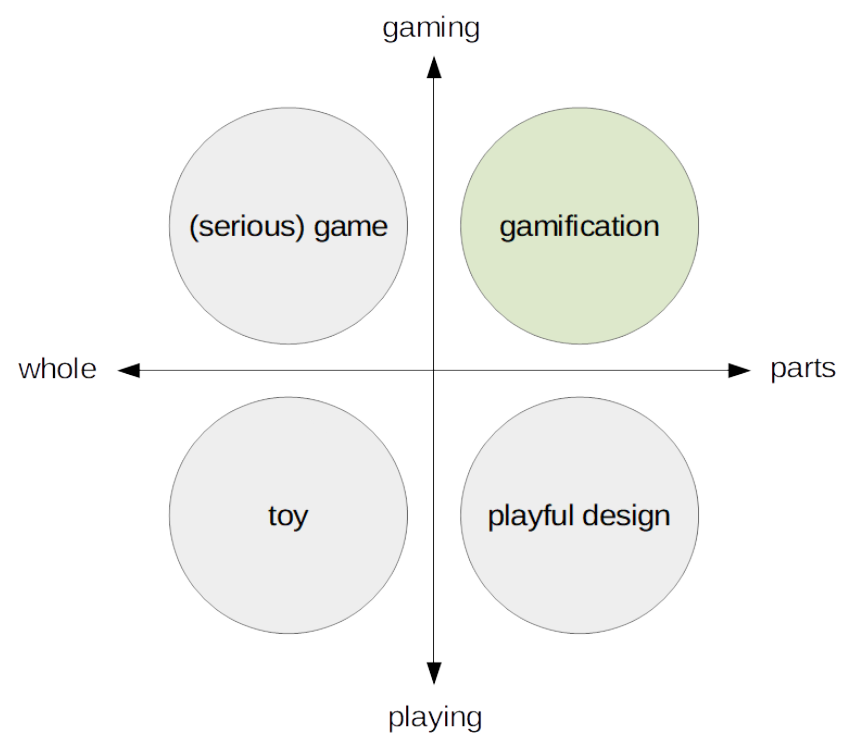
\includegraphics[width=0.5\linewidth]{images/dimensions.png}
    \caption{The dimensions of gaming/playing and whole/parts (After \cite{10.1145/2181037.2181040})}
\end{figure}

In order to distinguish gamification from game-based learning, gamification just introduces gamelike elements (elements or mechanics) into a non-gaming setting. Game-based learning, however, is a type of game play that has defined learning outcomes (Becker, 2021). With a specific learning goal in mind, a learning task is redesigned to make learning more interesting and more effective. This involves the use of serious games and elements of gamification in the learning process, seen as a tool of game-based learning. 

\subsection{Game Frameworks}
To date, educational game development teams have utilized a diverse mix of game design and instructional design methodologies to help realize their designs, but often without a unifying framework to bring these diverse perspectives together. An iterative approach to designing educational games is Winn's (2008) Game Design Play and Experience Framework, which is a modificaiton of the Mechanics, Dynamics, and Aesthetics (MDA) Framework as it does not address aspects outside of Entertainment. According to Figure 1.2, the designer of an educational game would usually have to take into account 4 different layers[17]. Learning, Storytelling, gameplay and user experience. This thesis focuses on the 3rd and 4th layer of the framework, gameplay and user experience.

\begin{figure}[H]
    \centering
    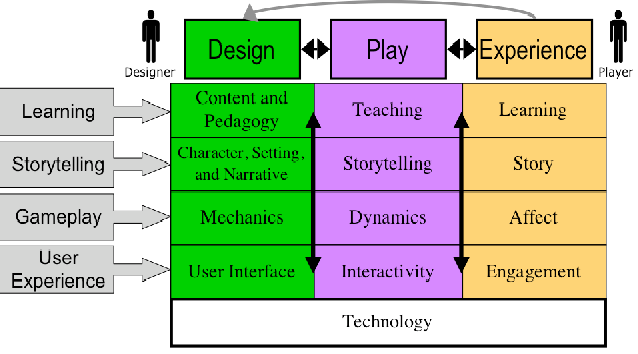
\includegraphics[width=0.5\linewidth]{images/dpe framework.png}
    \caption{Design, play and experience framework}
\end{figure}


The gameplay layer most closely resembles another framework. The gameplay layer defines what the player does in the game and is broken down into mechanics, dynamics and effects. The mechanics are the rules that define the operation of the game world, what the player can do, the challenges the player will face, and the player’s goals. The dynamics are the resulting behavior when the rules are instantiated over time with the influence of the
player’s interactions. The resulting experiences, or emotions derived in the player, are the affects. This is the rules and operations of the game world and the background processes of our game. For the purposes of the project, our focus on executing code is the core mechanic and dynamic of the game.

The user experience layer is designed so that user interfaces are made to access the entertaining gameplay (Saltzman, 2000, p. 256) and to create a vehicle to realize the desired serious outcomes. Good user interfaces are said to be transparent, that is, the player does not have to focus their attention on how to play the game (i.e., what button to press) but rather on the gameplay, storytelling, and learning experience.

The aspects of gameplay and user experience layer of the designer are key areas of game development concern that should also be implemented for educational games. The conceptualisation and implementation of such game elements/mechanics for the project will be explored in depth in later sections.

\subsection{Other educational games in Computer Science}
According to \cite{combefis2016learning}, there are mainly three categories of games in Computer Science:
\begin{itemize}
    \item \textbf{Coding}: The focus is to make users learn and train to code. Coding games require the learner to understand and to be able to write code to solve challenges. A central part is to understand the syntax behind a programming language.
    \item \textbf{Algorithmic thinking}: The focus is not on learning a particular programming language and relating concepts, but on learning concepts like algorithms and data structures. The system provides various problems that have to be solved in a technical way. This does not necessarily use programming languages, but can be done with other concepts.
    \item \textbf{Creating games}:  It is a kind of online programming learning platform that offers the possibility for the users to create their own games. On these platforms, the learner has to program a game, typically with a visual programming language. 
\end{itemize}			% 2. Literaturanalyse/Related work analysis
\newpage

\thispagestyle{myPageStyle}
\section{Basic Game Elements/Mechanics}
Game Mechanics function as basic systems of a game that governs their respective game elements (\cite{adams2012game}). All possible basic functions(represented by algorithms and data structures) and rules in the game are part of the mechanics. The section will discuss about planned game mechanics and their implementation.

\subsection{Web application}
The game will be a web application, this is because web applications are easily accessible and can be played on any device with a web browser. The game will be built using Angular, a popular web application framework. As central storing technique, MongoDB was used. This is because MongoDB is a NoSQL database, which is a good choice for storing JSON data. This database stores all relevant information regarding the
game content and the analytics


\subsection{Level selection}
The game will have multiple levels, each level will have a different set of challenges. The player will have to complete each level to progress to the next. The levels will be designed to increase in difficulty as the player progresses. The levels will be designed to teach the player different concepts of Python programming. The player will have to complete each level to progress to the next. The levels will be designed to increase in difficulty as the player progresses. The levels will be designed to teach the player different concepts of Python programming. The player will have to complete each level to progress to the next. The levels will be designed to increase in difficulty as the player progresses. The levels will be designed to teach the player different concepts of Python programming.





\subsection{Code Input}
The whole user flow of the educational game, game flow\cite{kramarzewski2018practical}, can be simplified. It starts out with the user input, which would be the code submitted, the process would be the gameplay mechanics and the output would be the reward for the player. 

This whole user experience starts with the user input, the submission of code can be done with a simple basic text box.
\begin{figure}[h]
    \centering
    
\includegraphics[width=0.5\linewidth]{images/textbox.png}
    \caption{Simple basic text box}
\end{figure}
\\\\
To improve on this submission of code, we can use a code editor like professional integrated development environments (IDEs). An in-browser code editor such as Monaco or ace editor would suffice; additional improvements to build upon a code editor with other options such as night/day mode, a language server to verify Python syntax formatting, and other such Python language features as it is not natively implemented within editors such as Monaco. Other features that should be implemented to help with user experience would be code completion, syntax/semantic highlighter, definition provider, formatting provider, and more.
\begin{figure}[H]
    \centering
    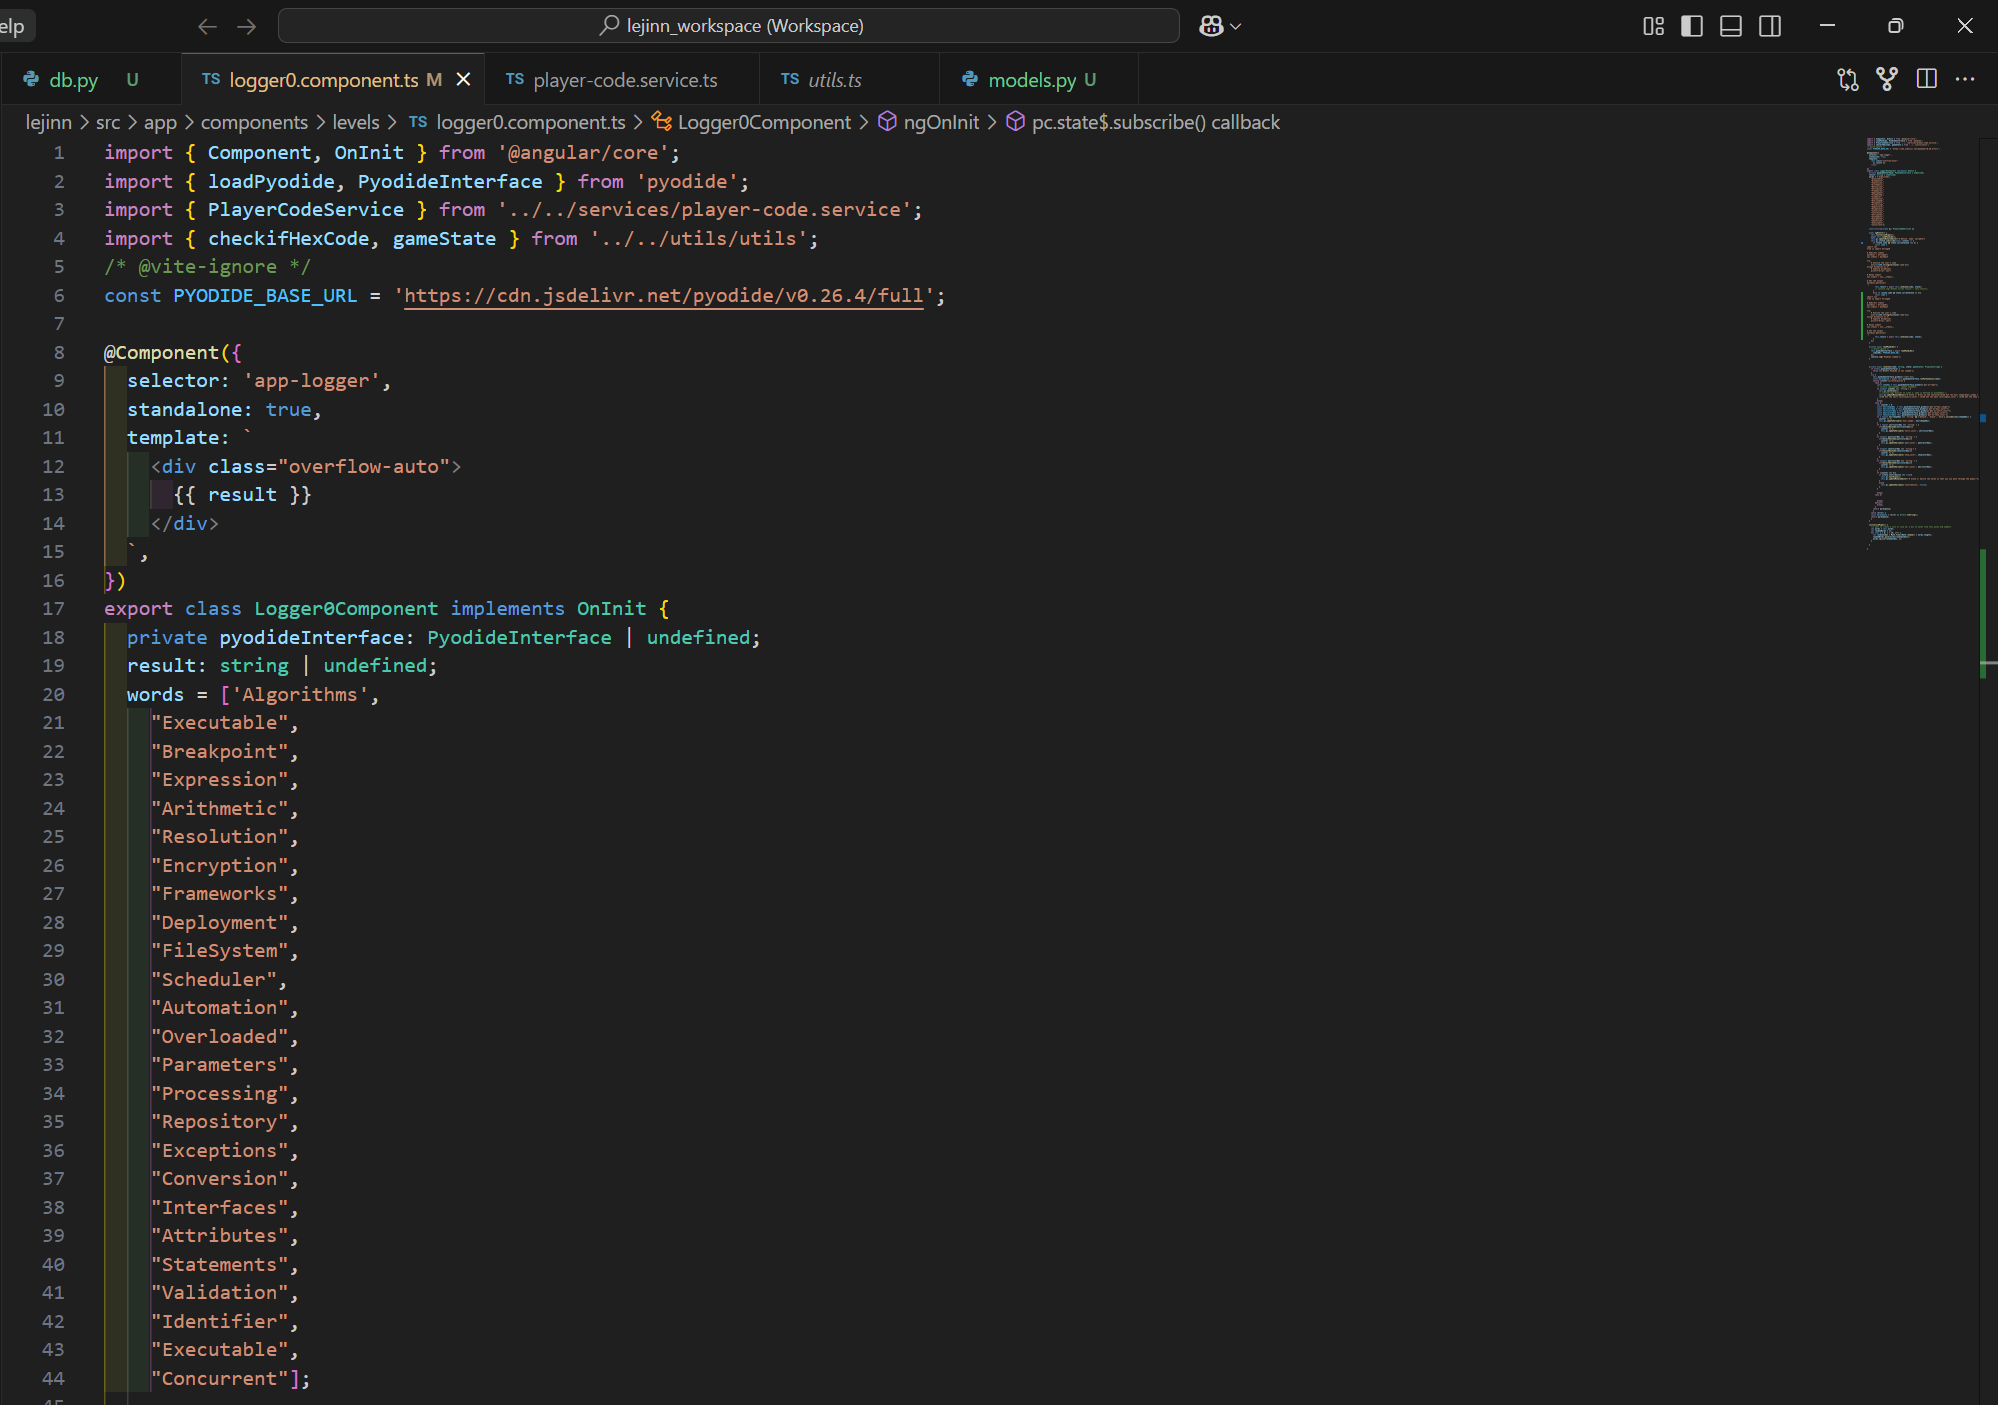
\includegraphics[width=0.3\linewidth]{images/code_editor.png}
    \caption{Code editor of IDE, a significant improvement over a basic textbox}
\end{figure}
Upon code submission, there is a reaction of the code that ran. This reaction of running code is usually known as standard output(stdout). This has to be printed out, including all results and any errors of the code. Other than just text printing with results of code submission, storytelling can take place here that is reactive upon successful results. 
		  % 3. Implementation, Technical Setting, Prototype
\newpage

\thispagestyle{myPageStyle}
\input{Chapter4/chap4}		% 4. ...
\newpage
\iffalse
\thispagestyle{myPageStyle}
\input{Chapter5/chap5}			% 5. ...
\newpage

\thispagestyle{myPageStyle}
\input{Chapter6/chap6}			% 6. Study design and execution
\newpage

\thispagestyle{myPageStyle}
\input{Chapter7/chap7}			% 7. Evaluation and Results
\newpage

\thispagestyle{myPageStyle}
\input{Chapter8/chap8}			% 8. Discussion, Deriving concrete action recommendations
\newpage

\thispagestyle{myPageStyle}	% 9. Conclusion, Future work, Limitations
\input{Chapter9/chap9}
\newpage
\fi	

	%\shorthandon{"}
	
%--------------------------------------------------------------------------------
%-----Anhang---------------------------------------------------------------------
%--------------------------------------------------------------------------------
	
	\pagenumbering{Roman} 					% Römische Nummerierung der Kapitel/Roman page numbering
	\setcounter{page}{6} 						% Beginn bei Seitenzahl X (hier: 6) um bei oberer Nummerierung aufzuschließen/Adapt page numbering
	
	%Glossar/Glossary
	\thispagestyle{myPageStyle}
	\glssetwidest{A D A S} 						% gleicher Abstand zur 2. Spalte (längstes Wort)					
	\setglossarystyle{alttree}																	
	%\printglossary[title=Abkürzungsverzeichnis,toctitle=Abkürzungsverzeichnis] 	% Rename for German thesis
	\cleardoublepage
		
	
	%Literaturliste/Literature references
	\thispagestyle{myPageStyle}
	\bibliographystyle{plainnat}
	%\bibliographystyle{abbrv}% changed abbrvdin to abbrv % DIN-Norm für Literaturdarstellung  plaindin 
	%\bibliographystyle{abbrvnat}
	\setcitestyle{authoryear, open={(}, close={)}}
	
	\renewcommand{\refname}{Literature references} % Remove for German thesis
	\bibliography{literature}					% Pfad und Datei der Literaturdatenbank/Path and file name of literature references
	\cleardoublepage	
	
	%Anhänge/Appendices
	%\thispagestyle{myPageStyle} 
	%\include{appendices}
	%\cleardoublepage
	
%----------------------------------------------------------------------------------
%----------------DOKUMENTENENDE - END OF DOCUMENT----------------------------------
%----------------------------------------------------------------------------------
	
\end{document}
